\section{Member 1: the expected-loss picture and the prior-shift experiment}
\label{sec:m1}
\textbf{Code:} \code{experiments/t1\_expected\_loss.py}, \code{experiments/task4\_prior\_shift.py}.

\paragraph{The decision rule in one picture.}
Figure~\ref{fig:t1} plots the expected cost of each action against $\post$. The cheapest action is
the lowest line. At $\ci=0.3$ the flat inspect line cuts off the peak where the other two cross,
giving the inspect band $(0.3,0.97)$. At $\ci=1$, above $\cstar=10/11$, it never does, and the rule
is the single cut at $10/11$.

\begin{figure}[!htbp]
\centering
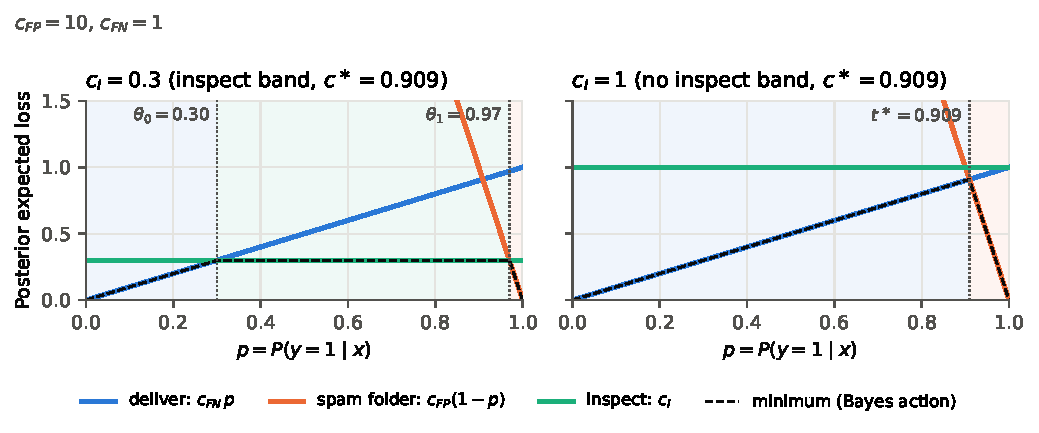
\includegraphics[width=0.92\linewidth]{t1_expected_loss.pdf}
\caption{Expected cost of delivering, filing as spam and inspecting against $\post$, for
$\cfp=10$, $\cfn=1$. Shading marks where each action is cheapest. Left: $\ci=0.3$. Right: $\ci=1$.}
\label{fig:t1}
\end{figure}

\paragraph{Does the prior correction work?}
The script tests Member 5's correction on data where only the spam rate changes, with
$\cfp=10$, $\cfn=1$, $\ci=0.3$. On synthetic data the models are trained at $\pio=0.5$ and tested on
fresh samples at each deployment rate $\pion$ from $0.05$ to $0.8$. On Spambase (trained at
$\pio=0.394$) the test part is resampled within each class to the new rate, for example $586$ emails
of which $29$ are spam at $\pion=0.05$. Both the shared Gaussian model and logistic regression are
used, and the decisions are made on four versions of $\post$: uncorrected, corrected with the true
$\pion$, corrected with $\pion$ estimated from the unlabelled test emails by the EM method of Saerens
et al.~\cite{saerens2002}, and (synthetic only) the true posterior.

\begin{figure}[!htbp]
\centering
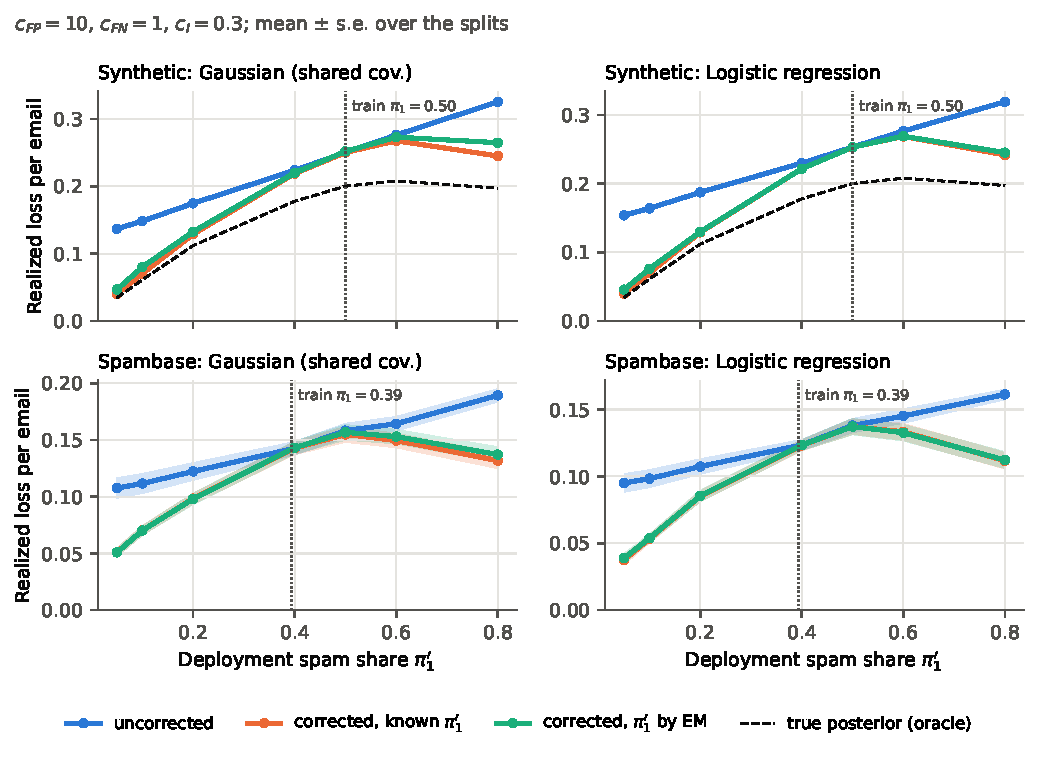
\includegraphics[width=0.88\linewidth]{c5_prior_shift.pdf}
\caption{Realized loss against the deployment spam rate $\pion$, without correction, with the known
$\pion$ and with $\pion$ estimated by EM (bands: $\pm1$ standard error over 20 splits). Dashed: the
true posterior. Dotted: the training rate.}
\label{fig:c5}
\end{figure}

\begin{table}[!htbp]
\centering\footnotesize
\input{\resultsdir/c5_loss_spambase.tex}
\caption{Spambase: realized loss after the spam rate changes to $\pion$ (training rate $0.394$),
without correction, corrected with the known $\pion$, and corrected with the EM estimate
(mean $\pm$ standard error, 20 splits).}
\label{tab:c5}
\end{table}

\paragraph{Results (Figure~\ref{fig:c5}, Table~\ref{tab:c5}).}
\begin{itemize}
  \item \emph{The correction pays off, and more so the larger the shift.} At $\pion=0.05$ it more than
        halves the loss: on Spambase from $0.095$ to $0.038$ (logistic) and from $0.108$ to $0.051$
        (Gaussian); on synthetic data from $0.154$ and $0.137$ to $0.040$, close to the $0.034$ of the
        true posterior. At the training rate the curves coincide, as they should.
  \item \emph{Where the saving comes from.} Without correction the filter still believes half of the
        synthetic emails are spam, so it inspects $43$--$49\%$ of them; after correction it inspects
        $1.6\%$. The corrected filter is slightly \emph{less} accurate ($96.4\%$ against $98.7\%$ on the
        emails it does not inspect) but three to four times cheaper.
  \item \emph{An unknown rate can be estimated if the model is calibrated.} For logistic regression on
        Spambase the EM estimate is off by $0.007$--$0.013$ on average and the loss is almost the same as
        with the true rate. The Gaussian model's estimate is too low: by $0.04$--$0.07$ on synthetic data,
        and by $0.036$--$0.047$ on Spambase once $\pion\ge0.4$.
\end{itemize}
